\section{Task 3}
  Um die Zeiten zu messen, haben wir eine einfache Stoppuhr Klasse implementiert. 
  Diese hat eine Auflösung im Bereich von Nanosekunden.

  Für die eigentliche Performance Messung haben wir die \textit{PerfLogger} Klasse entworfen.
  Mit dieser Klasse, können wir über die \textit{start-} und \textit{stopTotal()}-Methoden
  die Zeit messen, die insgesamt für einen Zug gebraucht wird. mit den \textit{start-} und
  \textit{stopInner()/stopLeaf()}-Methoden können wir Zeit messen, die einzelne Knoten
  brauchen. Dabei wird zwischen inneren Knoten und Blättern unterschieden. Blätter sind
  hierbei alle Knoten, auf denen die Evaluierungsfunktion ausgeführt wird.
  Außerdem inkrementieren diese Methoden einen Zähler, sodass wir wissen, wie viele Knoten
  welcher Art besucht wurden.
  Auch wird die gemessene Zeit gespeichert.  So lässt sich später dann die maximale, minimale
  und durchschnittliche Dauer berechnen.

  \subsection{Performance Vergleich}
    Wir haben auf einer Map 1000 mal in Folge den besten Move berechnen lassen, ohne dass
    sich die Map verändert, und die Performance Daten für jeden Zug gemessen. Die
    durchschnittlichen Ergebnisse sind in den Folgenden Diagrammen abgebildet:
    
    Wenn nicht in die Tiefe gerechnet wird, unterscheiden sich die beiden Algorithmen wenig.
    Der \textit{MinMax}-Algorithmus ist sogar minimal schneller,wie Abbildungen
    \ref{fig:time-1} und \ref{fig:node-1} zeigen.
    
    Ab einer Tiefe von 2 sind jedoch deutliche Unterschiede bemerkbar.
    Wie wir in Abbildung \ref{fig:time-2} sehen, braucht \textit{Alpha-Beta-Pruning}
    wesentlich weniger Zeit als der \textit{MinMax}-Algorithmus. In Abbildung
    \ref{fig:node-2} sehen wir auch den Grund dafür: Der \textit{Alpha-Beta}-Algorithmus
    besucht sehr viel weniger Blätter.
    
    Sobald bis Tiefe 3 oder weiter gerechnet wird, verdeutlicht sich das Bild, dass sich
    schon auf Tiefe 2 zeigte. Allerdings besuchter der \textit{Alpha-Beta}-Algorithmus nun
    auch weniger innere Knoten, wie Abbildungen \ref{fig:time-3} und \ref{fig:node-3} belegen.
    
    \begin{figure}[h]
      \centering
      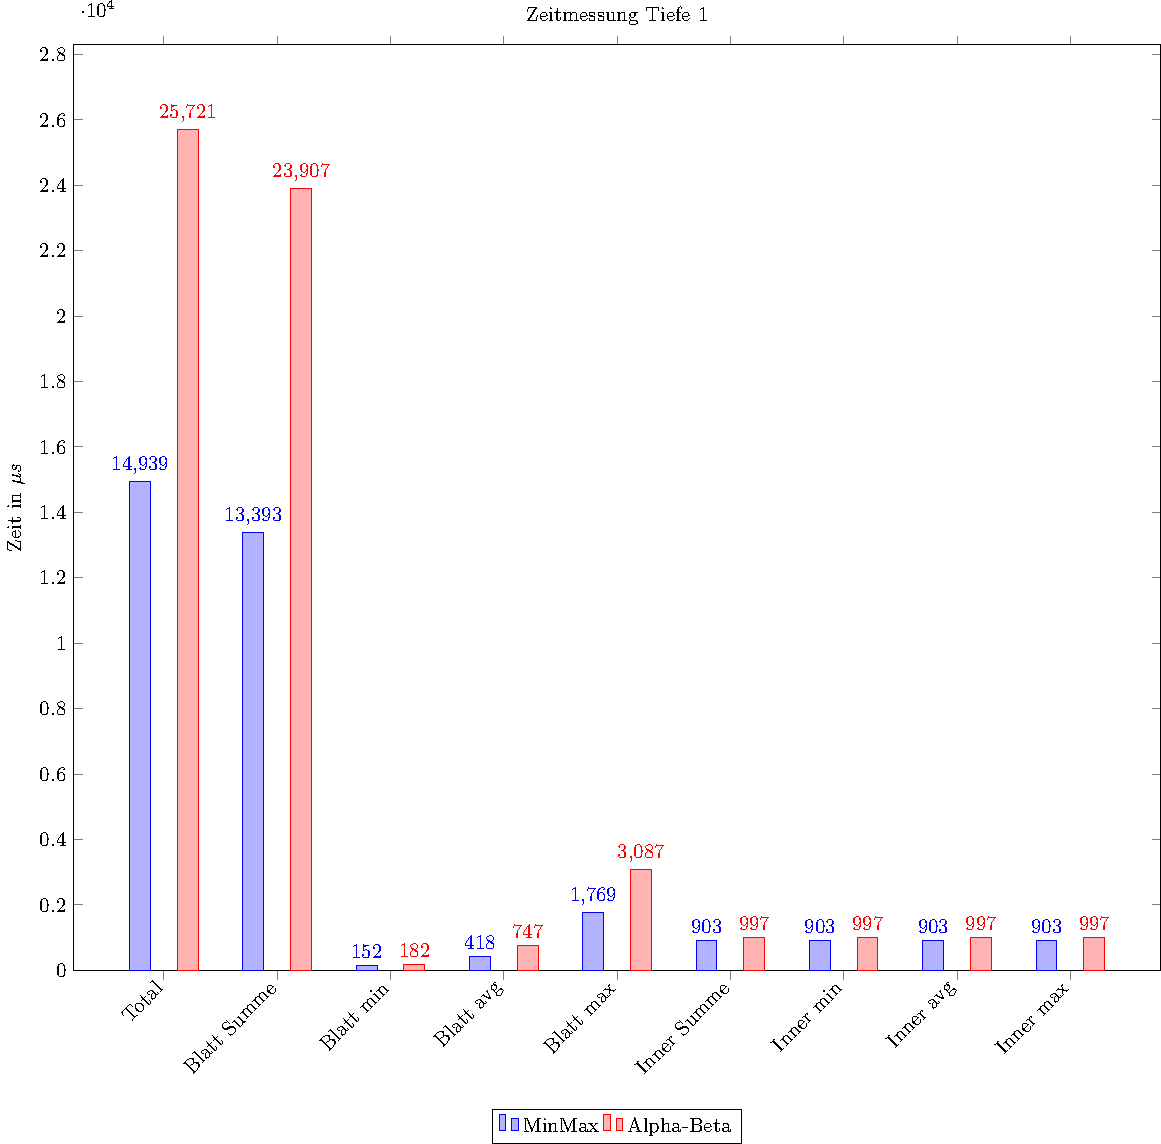
\includegraphics[width=\textwidth]{figures/time-1.pdf} 
      \caption{Gemessene Zeiten bei Rechnung bis Tiefe 1}
      \label{fig:time-1}
    \end{figure}
    \begin{figure}[h]
      \centering
      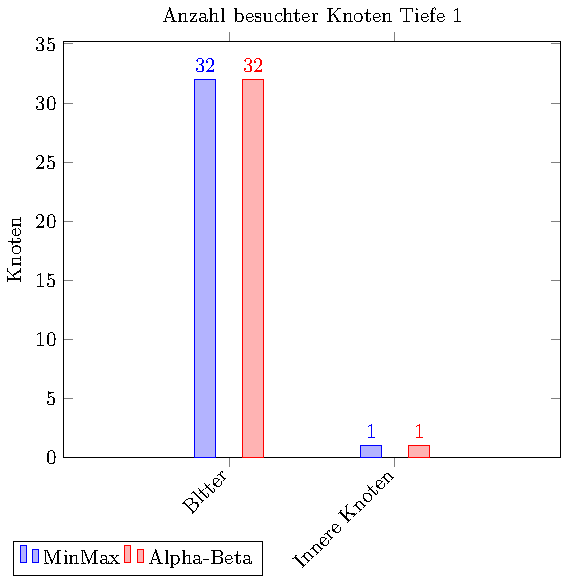
\includegraphics[width=\textwidth]{figures/node-1.pdf} 
      \caption{Anzahl besuchter Knoten bei Rechnung bis Tiefe 1}
      \label{fig:node-1}
    \end{figure}
    
     \begin{figure}[h]
      \centering
      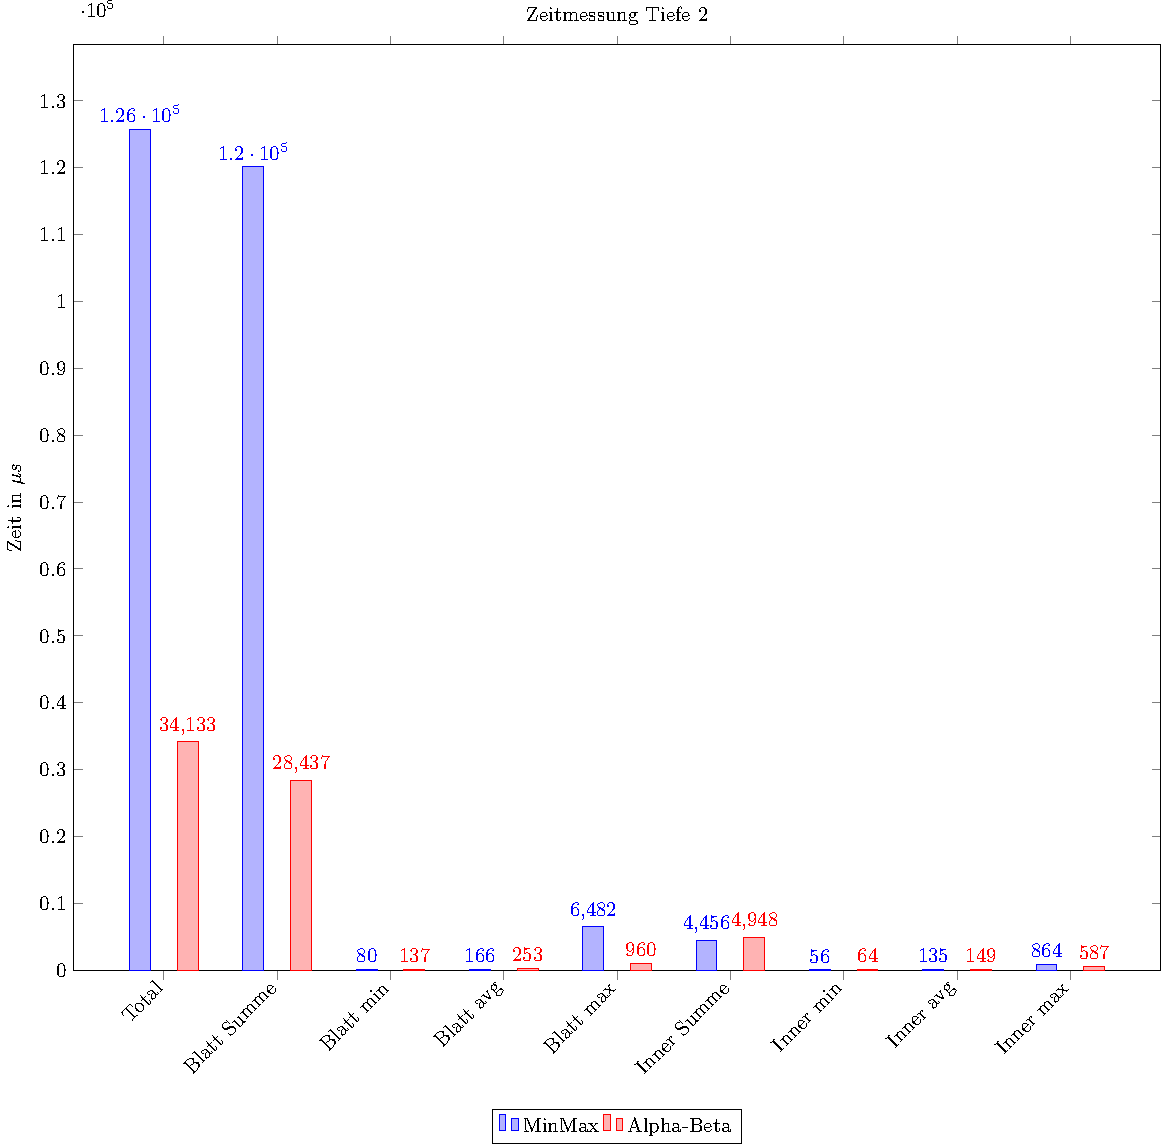
\includegraphics[width=\textwidth]{figures/time-2.pdf} 
      \caption{Gemessene Zeiten bei Rechnung bis Tiefe 2}
      \label{fig:time-2}
    \end{figure}
    \begin{figure}[h]
      \centering
      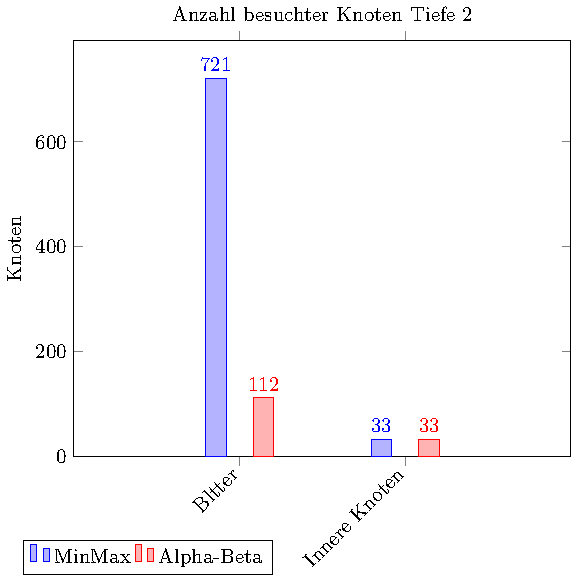
\includegraphics[width=\textwidth]{figures/node-2.pdf} 
      \caption{Anzahl besuchter Knoten bei Rechnung bis Tiefe 2}
      \label{fig:node-2}
    \end{figure}
    
     \begin{figure}[h]
      \centering
      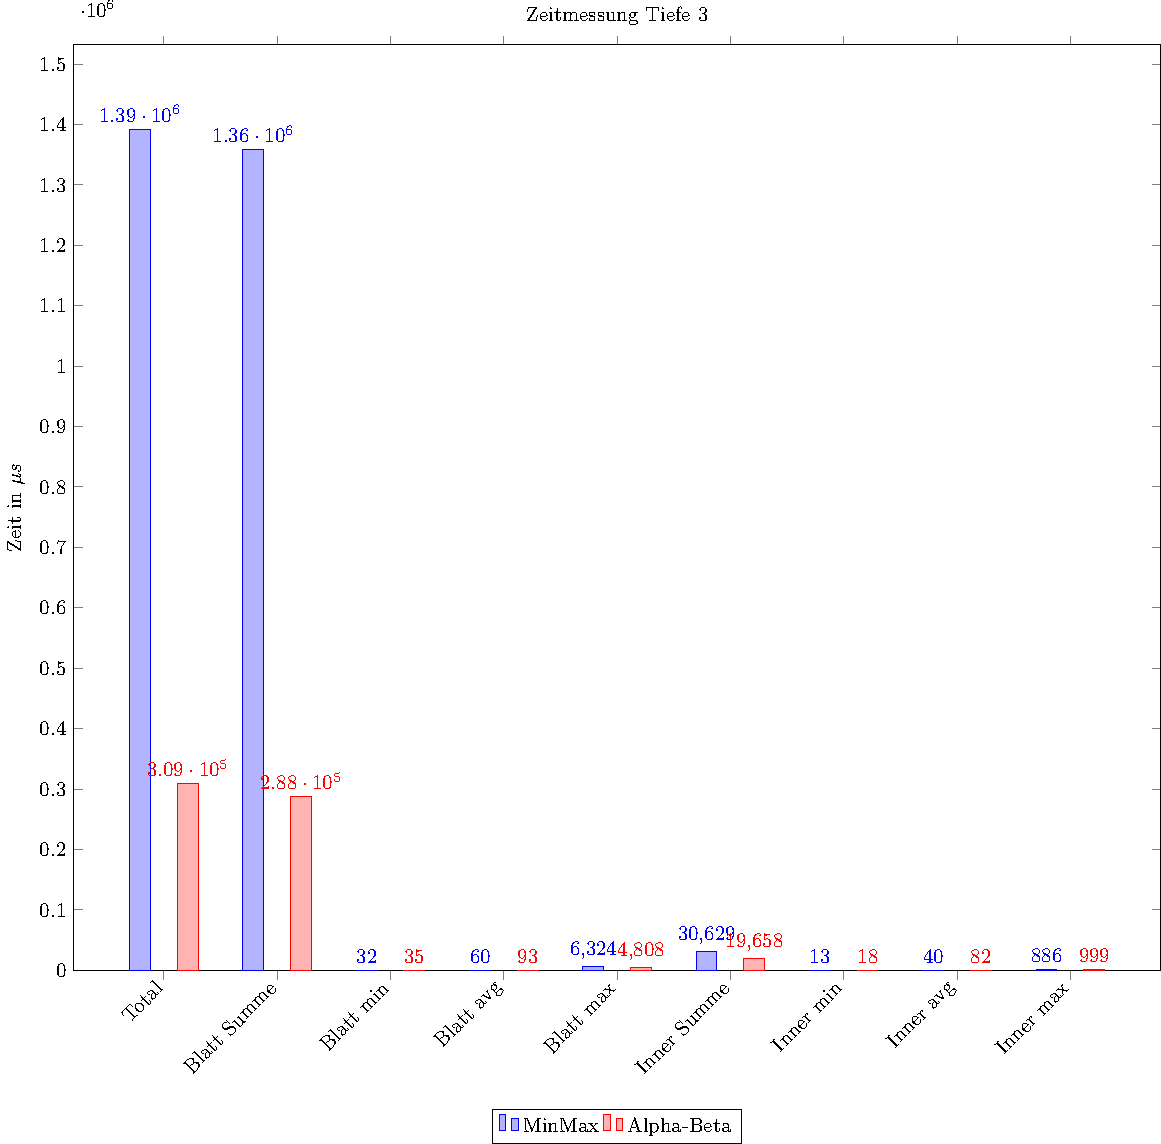
\includegraphics[width=\textwidth]{figures/time-3.pdf} 
      \caption{Gemessene Zeiten bei Rechnung bis Tiefe 3}
      \label{fig:time-3}
    \end{figure}
    \begin{figure}[h]
      \centering
      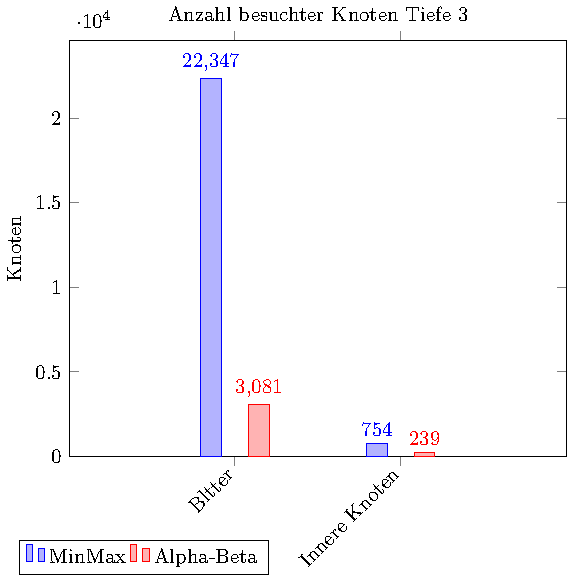
\includegraphics[width=\textwidth]{figures/node-3.pdf} 
      \caption{Anzahl besuchter Knoten bei Rechnung bis Tiefe 3}
      \label{fig:node-3}
    \end{figure}